\documentclass[anon]{CI}

% The following packages will be automatically loaded:
% amsmath, amssymb, natbib, graphicx, url, algorithm2e
\usepackage{adjustbox}
\usepackage{makecell}
\usepackage{multirow}

\makeatletter
\def\set@curr@file#1{\def\@curr@file{#1}} %temp workaround for 2019 latex release
\makeatother

\title[Ninjas’ Revenge]{Ninjas’ Revenge: the secret genetic technique}

 % Use \Name{Author Name} to specify the name.
 % If the surname contains spaces, enclose the surname
 % in braces, e.g. \Name{John {Smith Jones}} similarly
 % if the name has a "von" part, e.g \Name{Jane {de Winter}}.
 % If the first letter in the forenames is a diacritic
 % enclose the diacritic in braces, e.g. \Name{{\'E}louise Smith}

 % Two authors with the same address
  % \coltauthor{\Name{Author Name1} \Email{abc@sample.com}\and
  %  \Name{Author Name2} \Email{xyz@sample.com}\\
  %  \addr Address}

 % Three or more authors with the same address:
 % \coltauthor{\Name{Author Name1} \Email{an1@sample.com}\\
 %  \Name{Author Name2} \Email{an2@sample.com}\\
 %  \Name{Author Name3} \Email{an3@sample.com}\\
 %  \addr Address}


 % Authors with different addresses:
 \author{\Name{Cristian Andres {Camargo Giraldo}} \Email{cristian.andres.camargo@estudiantat.upc.edu}\\
 \AND
 \Name{Rodrigo Pablo {Carranza Astrada}} \Email{rodrigo.pablo.carranza@estudiantat.upc.edu}\\
 \AND
\Name{Santiago {del Rey Juárez}} \Email{santiago.del.rey@estudiantat.upc.edu}\\
 \AND
 \Name{Yazmina {Zurita Martel}} \Email{yazmina.zurita@estudiantat.upc.edu}\\
 }

\begin{document}

\maketitle

\begin{abstract}
This is a great project and therefore it has a concise abstract.
\end{abstract}

\begin{keywords}
Knapsack problem, Genetic Algorithms
\end{keywords}


\section{Problem statement and goals}

One of the most popular problems studied in constrained combinatorial optimization is the knapsack problem. Given a finite set of objects with associated weights and values, the objective is to maximize the value of a collection formed by these items without exceeding a predefined weight limit.

The knapsack problem has diverse practical applications which makes it particularly interesting. For example, it has been applied to production and inventory management \cite{ziegler1982solving}, financial models \cite{mathur1983branch} and queueing operations in computer systems \cite{gerla1977topological} or manufacturing \cite{bitran1989tradeoff}.

There are several variations to the knapsack problem. We could consider there are multiple copies of each item or take into consideration their volume in addition to their weight. However, we will focus on the simplest case, the one dimensional 0-1 knapsack problem, where the only constraint is the weight and the number of copies of each item is limited to 1.

Although the premise might look simple on the surface, this is actually an NP-hard problem. Thus, no known algorithm achieves optimal solutions in polynomial time for all cases of this problem. Still, a sufficiently good solution can be found quickly by resorting to heuristics methods. The one that we will explore is an effective and commonly used metaheuristic known as genetic algorithm.

Genetic algorithms (GAs) belong to the family of techniques known as evolutionary algorithms. They draw inspiration from natural selection and genetic processes to provide solutions to complex optimization problems and model evolutionary systems. 

The main process can be described as an evolutionary cycle. They first initialise a population of chromosomes, which represent candidate solutions. Some of these individuals will be drawn from the population through a selection mechanism and compared according to their fitness. In the reproduction phase, the genetic material of the best individuals will be combined to form offspring. Also, some values of the offspring’s chromosomes will be mutated. Finally, a replacement strategy is set to generate the next generation population. This process is repeated for several generations or until some convergence criterion is met.

We can describe formally the 0-1 knapsack problem as follows: given a set of $n$ items and a $knapsack$ with
\begin{center}
    $p_j = $ profit of item $j$, \\
    $w_j = $ weight of item $j$ \\
    $c = $ capacity of the knapsack, \\
\end{center}
select a subset of items so as to \\
\begin{center}
    maximize $z = \displaystyle \sum_{j=1}^n p_j x_j$ \\
    subject to $\displaystyle \sum_{j=1}^n w_j x_j < c,$ \\
\end{center}
where
$$x_j =     
    \begin{cases}
      1 & \text{if item $j$ is selected;}\\
      0 & \text{otherwise}
    \end{cases}, \hspace{1cm}
j \in N = \{1,..., n\}
$$


A solution to the knapsack problem can be represented as a sequence of binary values $[x_1, x_2, ..., x_n]$. We will apply GAs to eighteen different cases, each of them specified by a file containing a value for $n$ and $c$ in the first line and values for $p_j$ and $w_j$ in subsequent lines for each object $x_j$. \\

The goal of this project is to find the optimal solution to each of the eighteen knapsack problems proposed by applying GAs. To this end, we will have to choose and implement suitable mechanisms in each of the phases of the evolutionary cycle. The description of these methods, as well as the reasons for their election, are detailed in Section~\ref{sec:ci-methods}.

\section{Previous work}

This is a very important part, because it puts your work in context.

\section{The CI methods}\label{sec:ci-methods}
When applying genetic algorithms to a problem, there are several aspects to consider, each one with its own methods. In this section, we define the different methods used in our implementation for each one of these aspects.

\subsection{Population initialization}
For the initialization of the population, we have used a random initialization approach, which has been traditionally used in GAs for its simplicity and efficiency. However, we introduced an initialization range parameter to give the algorithm better chances of finding the optimal solution in case we know where this solution should be. This initialization range in conjunction with the possibility of sorting the input items by their value/weight rate can highly improve the algorithm performance.

\subsection{Fitness function and selection}
To be able to assess how well an individual (i.e. possible solution) fits our objective we must first define the fitness function. For our particular problem, we defined the following fitness function:

\begin{align*}
F(x) & =\begin{cases}
-\infty & if\:x\bullet w>c\\
x\bullet v & otherwise
\end{cases}
\end{align*}

\noindent, where $x$ is the bitstring representing the individual, $w$ is the list of item weights, $v$ is the list of item values and $c$ is the knapsack capacity.

Once we have the fitness function we are able to proceed to the selection step. We decided to implement the tournament and elitism selection methods for our algorithm. Particularly, we use a fixed value of $k=2$ for both tournament and elitism. We decided to use tournament selection instead of other methods such as standard roulette wheel or rank selection because of its simplicity and because seems to outperform the other approaches~\cite{razali2011genetic}. On the other hand, elitism was implemented because of its usage in the tournament selection method.

\subsection{Crossover and mutation}
Several crossover techniques can be applied in GAs such as one-point, 2-point, multi-point (with more than two cut points) and uniform crossovers. In this work, we have implemented the one-point, 2-point and uniform crossovers. The reason behind this choice is the simplicity of these techniques and their good performance, especially the 2-point crossover~\cite{HASANCEBI2000435, dejonganalysis, adeli1993integrated}.

For the mutation step, we implemented a simple bit-flip where a random number of genes between 1 and the size of the chromosome are flipped. In addition, we set the mutation probability to 0.5 since lower values made the algorithm get stuck in local minimums more frequently.

\subsection{Replacement strategy}
The final step of the GA is the replacement strategy used to obtain the new generation. In our case, we used elitism to replace the worst individuals of the current population. With this strategy, the old generation might be entirely replaced. In addition to the elitism, we also decided to remove repeated individuals before applying the replacement. This decision was made to ensure that the diversity of the population is maintained. Additionally, we defined an extra case that does not use elitism. This is when there is no good solution (i.e. the fitness value is $-\infty$) neither in the parents nor the offspring. In this case, we decided to obtain the new generation by selecting, randomly, half of the individuals from $\mu$ and the other half from $\lambda$.

\section{Results and Discussion}
The main objective of this project was to implement a genetic algorithm that was able to achieve optimal, or near-optimal, solutions for the knapsack problem in a reasonable amount of time when compared with the exhaustive search method. To achieve this, we tried different methodologies such as sorting the items by their value/weight ratio or by using different crossover methods.

First, we started by comparing the three crossover methods implemented (i.e. one-point, two-point and uniform). In Table~\ref{tab:comparison}, we can see the results obtained with each method in three different problem sizes. We can see how the worst method,  in terms of finding the solution, is the one-point crossover since it is only able to find it for small sizes of the problem. The uniform crossover seems to outperform the two-point crossover method both in execution time and the number of times the best solution is found for small and medium-size problems. However, the two-point method is the only one able to find the best solution for the three files. Although these results are not concluding since we have not tested enough sizes, we think that this might indicate that for small and medium-sized problems the usage of uniform crossover should be preferred over the other two options and the two-point method should be used when we have a greater problem size.

\begin{table}[htbp]
    \centering
    \begin{adjustbox}{max width=\textwidth}
    \begin{tabular}{|c|c|c|c|c|c|c|c|}
    \hline 
    \multirow{2}{*}{Sol} & \multirow{2}{*}{\#items} & \multicolumn{2}{c|}{One-point } & \multicolumn{2}{c|}{Two-point} & \multicolumn{2}{c|}{Uniform}\\
    \cline{3-8}
     &  & Time (s) & Best found & Time (s) & Best found & Time (s) & Best found\\
    \hline 
    6 & 50 & 56.206 & 1/3 & 76.890 & 1/3 & 65,544 & 2/3\\
    \hline 
    9 & 100 & 131.852 & 0/3 & 109.723 & 1/3 & 43.720 & 3/3\\
    \hline 
    14 & 300 & 114.531 & 0/3 & 270.457 & 1/3 & 121.396 & 0/3\\
    \hline 
    \end{tabular}
    \end{adjustbox}
    \caption{Comparison between implemented crossover methods using the sort option,
    10000 max generations, 600 stall generations, a population size of
    $max(\#items^{2},2000)$ and tournament selection.}
    \label{tab:comparison}
\end{table}

Once we tested the different crossover methods, we proceeded to compare the algorithm without sorting the items by value/weight rate and with the sorting. To be able to compare them we fixed the set of parameters to avoid biasing the results as much as possible.

Looking at Table~\ref{tab:results}, it is possible to observe the following:
\begin{enumerate}
    \item It was possible to get the optimal value for $\sim89\%$ of the files tried.
    \begin{enumerate}
        \item For sol\_17 and sol\_18 we obtained sub-optimal solutions close to the optimal solution but due to the restriction of stall generations, the algorithm was not able to produce better results.
    \end{enumerate}
    
    \item There is a strong correlation between the number of items and the time it takes to find the optimal solution. That is, a Pearson correlation of 0.9873 for the runs without sort and 0.9979 for the runs with sort. However, certain files do not follow this trend. For instance, if we compare the results from sol\_12 and sol\_3 we see how the problem with more items (i.e. sol\_12) needs more or less the same time as the solution with fewer items (i.e. sol\_3) and even finds the optimal with more frequency. This is a behaviour that we would usually not expect.
    
    \item Sorting the items using their value/weight ratio helped to improve the time required to find the optimal solution significantly. In some cases, the improvement achieved is $\sim56$ times faster than the not sorted result. The mean speedup is around $\sim6$ times.
\end{enumerate}

\begin{table}[htbp]
    \centering
    \begin{adjustbox}{max width=\textwidth}
    \begin{tabular}{|c|c|c|c|c|c|c|c|}
    \hline 
    Sol & \#items & Best value & \makecell{Best value\\found} & \makecell{Time\\without sort (s)} & Best found & \makecell{Time\\with sort (s)} & Best found\\
    \hline 
    1 & 4 & 19  & 19  & 0.0378 & 4/4 & 0.0375 & 4/4\\
    \hline 
    2 & 19 & 12248 & 12248 & 2.445 & 4/4 & 0.430 & 4/4\\
    \hline 
    3 & 30 & 99798  & 99798  & 34.501 & 0/3 & 24.437 & 2/3\\
    \hline 
    4 & 40 & 99924  & 99924  & 4.382 & 3/3 & 0.674 & 3/3\\
    \hline 
    5 & 45 & 23974  & 23974  & 117.021 & 1/3 & 2.102 & 3/3\\
    \hline 
    6 & 50 & 142156  & 142156  & 247.373 & 0/3 & 76.890 & 1/3\\
    \hline 
    7 & 50 & 5345  & 5345  & 73.624 & 3/3 & 18.885 & 3/3\\
    \hline 
    8 & 60 & 99837  & 99837  & 12.803 & 3/3 & 34.425 & 3/3\\
    \hline 
    9 & 100 & 99837  & 99837  & 94.960 & 0/3 & 109.723 & 1/3\\
    \hline 
    10 & 100 & 1333930  & 1333930  & 321.234 & 0/2 & 23.198 & 2/2\\
    \hline 
    11 & 100 & 10892  & 10892  & 322.240 & 1/2 & 128.105 & 1/2\\
    \hline 
    12 & 200 & 100236  & 100236  & 49.784 & 2/2 & 24.183 & 2/2\\
    \hline 
    13 & 200 & 1103604  & 1103604  & 632.185 & 0/2 & 512.575 & 1/2\\
    \hline 
    14 & 300 & 1688692  & 1688692  & 417.575 & 0/2 & 196.617 & 1/2\\
    \hline 
    15 & 400 & 3967180  & 3967180  & 216.064 & 0/2 & 258.675 & 1/2\\
    \hline 
    16 & 500 & 54939  & 54939  & 614.917 & 0/2 & 191.009 & 1/2\\
    \hline 
    17 & 1000 & 109899 & 109894 & 699.159 & 0/2 & 643.658 & 0/2\\
    \hline 
    18 & 10000 & 1099893 & 1099132 & 4548.846 & 0/1 & 7,208.676 & 0/1\\
    \hline 
    \end{tabular}
    \end{adjustbox}
    \caption{Comparison between the algorithm using with the sort option or without
    it using 10000 max generations, 600 stall generations, a population
    size of $max(\#items^{2},2000)$, tournament selection and two-point
    crossover.}
    \label{tab:results}
\end{table}

It is interesting to find that sorting the items by their value/weight ratio yielded excellent results. We think that the reason is that sorting the items makes the best ratios to be found in the lower section of the bitstring (i.e. the bits belonging to the right half). If we combine this with a relatively small population range it is possible to get the first generation with a high fitness value and even it is possible to find the optimal solution amidst the initial generation. In the reproduction step, having this configuration helps next generations to improve their fitness score faster. This can be observed in the time required to find the solution in all the files tried. There might be some cases where the best solution is found by combining low value/weight ratio items or that there is not much difference in ratio between items. This could cause the sorting to have a lower impact on the final performance but still higher than the no sorting option.

Regarding the evolution of the fitness value throughout the different generations, most of the plots obtained (can be found in the submitted project) share the same trend. The fitness tends to flatten at the beginning after a few epochs/generations when a high value is reached. The flattening happens because we keep the best value found in subsequent iterations. However, we think that because of the mutation process that happens in each generation the GA can break out and find even higher fitness values. This can be observed in the graphics by the layered shape obtained. As an example, Figure~\ref{fig:fitness-evol} shows the fitness progression for the last file ninja\_18\_10000 where 10000 items were used.

\begin{figure}[htbp]
\floatconts
{fig:fitness-evol}
{\caption{Evolution of the fitness value for the ninja\_18\_10000 file using the sort option, 10000 max generations, 600 stall generations, a population
    size of 2000, tournament selection and two-point
    crossover.}}
{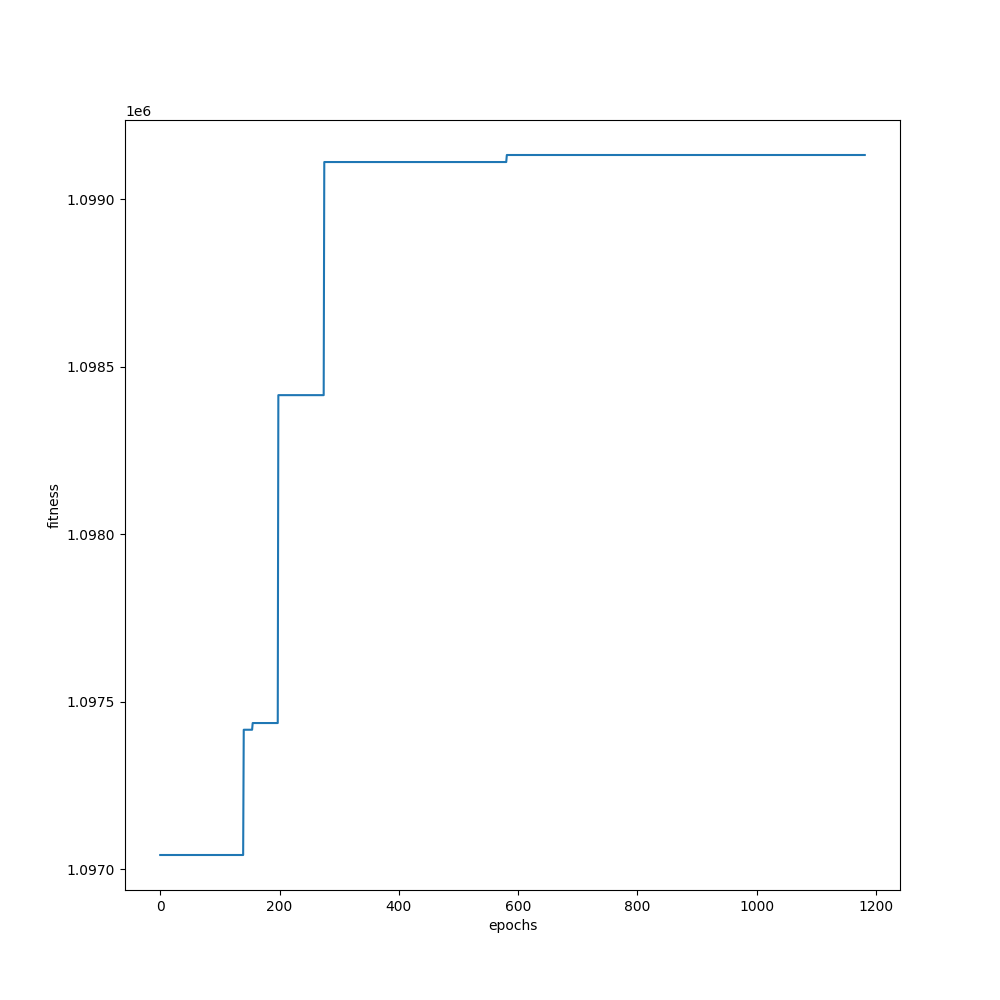
\includegraphics[width=.6\textwidth]{images/ninja_18_10000}}
\end{figure}


\section{Strengths and weaknesses} \label{sec:strengths}

After seeing the results obtained from our GA implementation we have detected some strengths and weaknesses in it.

Starting with its strengths, we have seen how the algorithm can find the optimal solution in a reasonable amount of time in most cases. This is a very good result since we usually would expect to obtain sub-optimal results. Also, we noticed that the algorithm can find multiple optimal solutions for some of the problems. Being able to find several optimal solutions to one problem opens the possibility to introducing new factors when deciding which one best suits us. This can be considered a strength compared to the standard exhaustive search algorithm since the latter is only able to find one possible solution. Another strong point of our solution is its simplicity since it does not require complex functions or procedures to achieve good results. We consider that this makes the algorithm easy to understand and extensible to other problems that can be represented as bitstrings.

Following with its weaknesses, we have seen how the algorithm struggles when the size of the problem increases dramatically (e.g. 1000 or 10000 items). In these cases, we observed how the exhaustive search outperformed our algorithm in terms of solution quality and time complexity since it could find the optimal solution in less time. Also, for some problems, we observed how successive executions performed considerably different when looking at the execution time and the solution obtained. From this, we infer that the GA is highly dependent on the initialization of the initial population.

\section{Conclusions and future work}

The genetic algorithm implemented has proven to be a good heuristic for generating approximate solutions of the unidimensional 0-1 knapsack problem. The results achieved were optimal or near-optimal in the eighteen scenarios studied despite the imposition of stopping criteria. 

We noted how the performance of the system improves drastically when the data is preprocessed suitably. Having a good understanding of the problem representation and the internal mechanisms in a GA is essential for this preliminary step.

Another aspect that determines the performance of the system is, of course, the strategies implemented in each phase of the evolutionary cycle. We counted with several methods to choose from at each step which makes these systems very flexible and adaptable. This along with a proper selection of parameters allowed us to tailor the algorithm to the problem.

There are ways to further optimize the developed method. As we mentioned earlier, GAs are highly sensitive to the population seeding technique. The random initialization of the population can generate individuals with poor fitness, which increases the time needed to achieve optimality. Instead, we could resort to better seeding techniques such as Sorted Population ~\cite{yugay2008hybrid}, which creates a large initial population, sorts it in ascending order according to their fitness and chooses a percentage of individuals that have above average fitness. \cite{hassanat2018improved} described and compared this and other initialization techniques like Nearest Neighbour or Gene Bank.

As we have seen in Section~\ref{sec:strengths}, one of the main weaknesses of our algorithm is that its execution time increases dramatically with the problem size. One way to slightly improve this issue could be to parallelize the reproduction process. In this way, we could randomly split the population into multiple batches and then perform the reproduction step simultaneously for each batch. With this, we only would need to wait for the slowest batch to finish and then join all the resulting offspring together to perform the replacement step.


\clearpage

\bibliography{references.bib}

\end{document}
